\documentclass[preprint,numbers,10pt]{sigplanconf}

\usepackage{graphicx}

\begin{document}

\title{Language Workbench Challenge 2016: Jetbrains MetaProgramming System}

\authorinfo{Eugen Schindler}{}{eugenschindler@gmail.com}
\authorinfo{Klemens Schindler}{}{klemensschindler@gmail.com}
\authorinfo{Federico Tomassetti}{Independent}{federico@tomassetti.me}
\authorinfo{Markus V\"{o}elter}{}{voelter@gmail.com}
\authorinfo{Kolja Dummann}{}{k.dummann@gmail.com}
\authorinfo{Remi Bosman}{}{remi.bosman@gmail.com}
\authorinfo{Ana Maria \c{S}ut\^{i}i}{}{farcasia@gmail.com}

\maketitle

%%%%%%%%%%%%%%%%%%%%%%%%%%%%%%%%%%%%%%%%%%%%%%%%%%%%%%%%%%%%%%%%%%%%%%%%%%%%%%%
%
% Introduction
%
%%%%%%%%%%%%%%%%%%%%%%%%%%%%%%%%%%%%%%%%%%%%%%%%%%%%%%%%%%%%%%%%%%%%%%%%%%%%%%%

\section{Introduction}

The Jetbrains MetaProgramming System is a mature Language Workbench based on projectional editing. While other Language Workbenches are based on projectional editing Jetbrains MPS is arguably the most mature, with a growing user base.

TODO: Describe how MPS does w.r.t. the feature model presented in Erdweg2015

TODO: Summarize results of MPS in previous challenges

\subsection{Structure of the paper}

\cite{erdweg2015evaluating}

%%%%%%%%%%%%%%%%%%%%%%%%%%%%%%%%%%%%%%%%%%%%%%%%%%%%%%%%%%%%%%%%%%%%%%%%%%%%%%%
%
% Notation Section
%
%%%%%%%%%%%%%%%%%%%%%%%%%%%%%%%%%%%%%%%%%%%%%%%%%%%%%%%%%%%%%%%%%%%%%%%%%%%%%%%

\section{Addressing the Notation Problem}

\subsection{Assumptions}

\subsection{Implementation}

\subsubsection{Support mathematical symbols in addition to textual notation}
\subsubsection{Support tabular notation in addition to textual notation}
\subsubsection{Support diagrammatic notations in addition to textual notation}
\subsubsection{Generic metadata annotations: annotation of program elements without changing their core meaning}
\subsubsection{Optional hiding: hide parts of the code, without losing the content and while retaining editability}
\subsubsection{Alternative notations: multiple notations for the same language}
\subsubsection{Computed properties: read only annotations that are automatically derived form the main program}
\subsubsection{Computed structures: structured, editable views}
\subsubsection{Skeleton editing: guide the user with syntactic templates with editable holes}
\subsubsection{Embedding code in prose: mix structured code with free text}
\subsubsection{Embedding blackboxes: allow program elements to be opaque non-textual elements}

\subsection{Variants}

\subsection{Usability}

\subsection{Impact}

\subsection{Composability}

\subsection{Limitations}

\subsection{Uses and examples}

\subsection{Effort (best-effort)}

\subsection{Other comments}

\subsection{Artifact}

%%%%%%%%%%%%%%%%%%%%%%%%%%%%%%%%%%%%%%%%%%%%%%%%%%%%%%%%%%%%%%%%%%%%%%%%%%%%%%%
%
% Evolution and Reuse Section
%
%%%%%%%%%%%%%%%%%%%%%%%%%%%%%%%%%%%%%%%%%%%%%%%%%%%%%%%%%%%%%%%%%%%%%%%%%%%%%%%

\section{Addressing the Evolution and Reuse Problem}

\subsection{Assumptions}

\subsection{Implementation}

\subsubsection{Language extension: modularly extend a language with new syntactic constructs}

In this section, we are going to describe the mbeddr language for state
machines with event-driven execution. The mbeddr state machines extends
the base language from MPS. This enables a seamless integration between
C code and state machine specifications.

State machines are a mathematical model of computation often used in embedded software
for describing discrete behaviour through state transitions. Its characterizing
ingredients are states, transitions and events. At any given time, a state
machine is in a state and it can be transitioned from one state to another.
A transition in a state machine is triggered by an event. These events
are usually provided by the environment, and, hence, the state machine
needs to have a way to interact with the environment. Besides events,
transitions can also have different guard expressions that need to hold when
the event arrives, for the transitions to be triggered.

We are now going to describe the extension of mbeddr with new syntactic notations for state machines.

In mbeddr, the state machine language is packaged in a language module and it
extends the base language of MPS. The \emph{StateMachine} concept extends
\emph{BaseConcept}, which means that the state machine is a program node,
as \emph{BaseConcept} is the concept from which all other concepts are derived.
The state machine language also implements the \emph{IModuleContent} interface,
which means that they can be top-level components in modules or can be inside of any
container that expects \emph{IModuleContent} children. Modules in mbeddr C
introduce basic program modularization, visibility control and namespaces \cite{voelter2013mbeddr}.

In the next paragraphs, we are going to present excerpts from a state machine for
judging flights. The state machine awards points for successful
takeoff and landing and for speed flown \cite{voelter2014generic}.

The state machine adds custom notation for specifying the state machine. The textual
form of the state machine can be seen in Figure \ref{HFAT}. The figure depicts a hierarchical state machine
that computes the points for a flight.
In addition, because textual forms can live alongside graphical and tabular forms in MPS, 
the state machine can be viewed in table form and graphical form as well alongside the piece of C code
where it is used. Figure \ref{HFATab} shows the same state machine for flight analyzes in tabular form.

\begin{figure}[ht!]
\centering
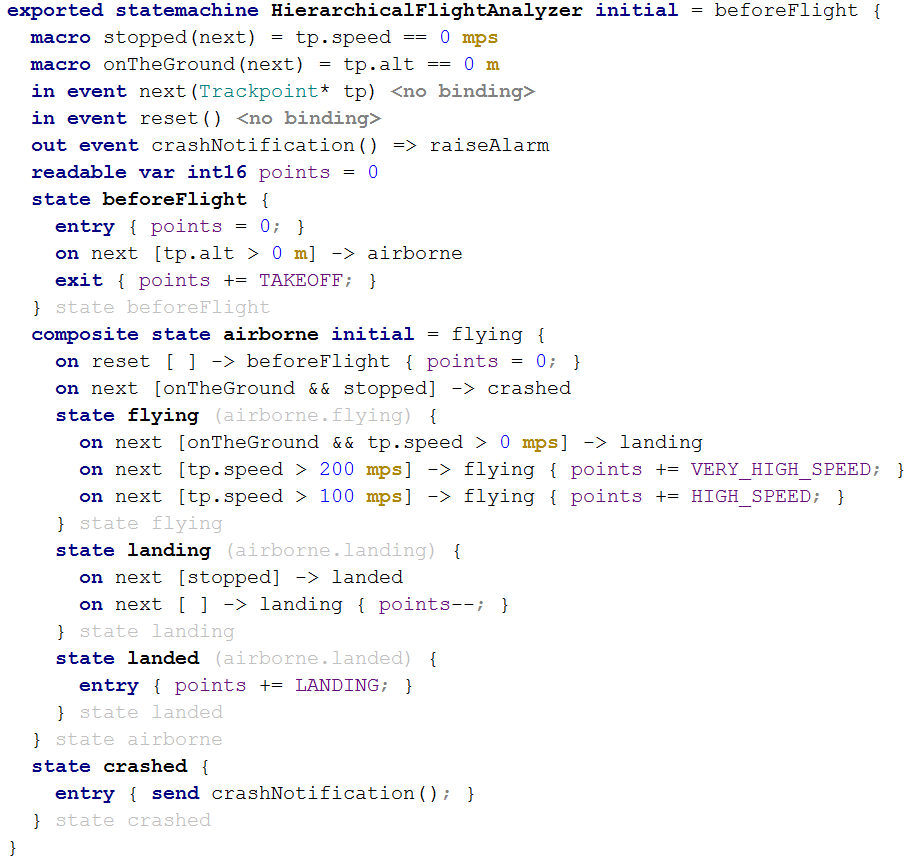
\includegraphics[scale=0.5]{figures/HierarchicalFlightAnalyzerT}
\caption{Hierarchical flight analyzer state machine - textual notation}
\label{HFAT}
\end{figure}

\begin{figure*}[ht!]
\centering
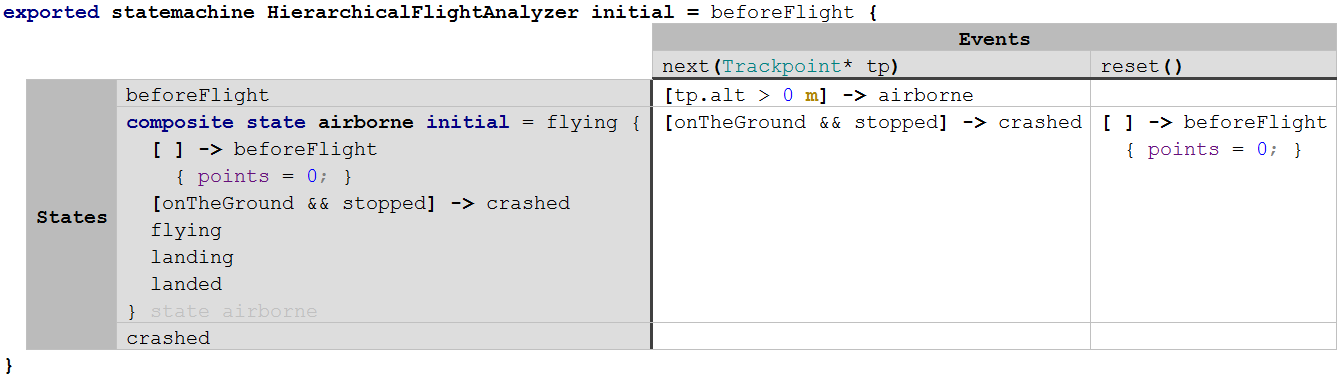
\includegraphics[scale=0.55]{figures/HierarchicalFlightAnalyzerTab}
\caption{Hierarchical flight analyzer state machine - tabular notation}
\label{HFATab}
\end{figure*}

Moreover, the state machine itself embeds arbitrary code in the actions
and in the guards. The actions are statement lists and the guards are expressions.
For instance, look at the guards and actions in Figure \ref{HFAT}; they contain mbeddr C expression.

\subsubsection{Language embedding: embed a separate language inside another}
\subsubsection{Extension composition: combine independently developed extensions}
\subsubsection{Beyond grammar restrictions: disallow constructs in certain scopes, without modeling this in the (abstract) syntax}
\subsubsection{Syntax migration: support migrating programs when concrete syntax changes}
\subsubsection{Structure migration: support migrating programs when abstract syntax changes}

\subsection{Variants}

\subsection{Usability}

\subsection{Impact}

\subsection{Composability}

\subsection{Limitations}

\subsection{Uses and examples}

\subsection{Effort (best-effort)}

\subsection{Other comments}

\subsection{Artifact}

%%%%%%%%%%%%%%%%%%%%%%%%%%%%%%%%%%%%%%%%%%%%%%%%%%%%%%%%%%%%%%%%%%%%%%%%%%%%%%%
%
% Editing Section
%
%%%%%%%%%%%%%%%%%%%%%%%%%%%%%%%%%%%%%%%%%%%%%%%%%%%%%%%%%%%%%%%%%%%%%%%%%%%%%%%

\section{Addressing the Editing Problem}

\subsection{Assumptions}

\subsection{Implementation}

\subsubsection{Editing incomplete programs: support for syntactically malformed programs}
\subsubsection{Referencing missing items: support referencing items that have not been defined}
\subsubsection{Structure agnostic copy-paste: copy-paste works across syntax boundaries}
\subsubsection{Restructuring: changing syntactic structure without typing the complete expression again.}
\subsubsection{Language demarcation: show how a combination multiple languages in one program are disambiguated}
\subsubsection{Delayed decisions: show when the syntactic category of an expression is determined}
\subsubsection{End-user defined formatting: show if and how user can change the visual appearance of the program}
\subsubsection{Specification of default formatting: support for pretty printing}
\subsubsection{Formatting preservation: how is formatting preserved when the code is automatically restructured}

\subsection{Variants}

\subsection{Usability}

\subsection{Impact}

\subsection{Composability}

\subsection{Limitations}

\subsection{Uses and examples}

\subsection{Effort (best-effort)}

\subsection{Other comments}

\subsection{Artifact}

%%%%%%%%%%%%%%%%%%%%%%%%%%%%%%%%%%%%%%%%%%%%%%%%%%%%%%%%%%%%%%%%%%%%%%%%%%%%%%%
%
% Conclusions
%
%%%%%%%%%%%%%%%%%%%%%%%%%%%%%%%%%%%%%%%%%%%%%%%%%%%%%%%%%%%%%%%%%%%%%%%%%%%%%%%

\section{Conclusions}

%% We are using the command `bibtex' from within the directory `build', thus we need
%% to go back from this directory and look for the bibliography file.
\bibliographystyle{plain}
\bibliography{../LWC2016}

\end{document}
